We start from the analytical benchmark of Section \ref{mms1} and we use $Q_1 \times P_0$
elements with a penalty formulation. 
We have seen in the first stone how to recover the elemental pressure as a postprocessing step. 
However, the discontinous nature of the pressure field (and the presence of a
parasitic checkerboard mode) can be problematic for many reasons 
(pressure enters the rheology, plotting , ...) . 
We then wish to project the elemental pressure onto the nodes of the mesh. 

Terminology: in general, when a discontinuous elemental pressure is used in a stone, 
it is called $p$ while its projection onto the nodes is coined $q$. 
In this case we compute several nodal pressures:
\begin{itemize}
%...........
\item $q_1$ is smoothed pressure obtained with the  center-to-node approach. We loop 
over  elements and each element adds its pressure to its corner nodes. Interior nodes 
'receive' 4 values, edge nodes 2 values and corner nodes only 1. An average per node
is then computed. This is a very simple and cost-effective method and it is used in 
papers based on DOUAR or FANTOM \cite{brtf08,thfb08,thie11}.

\begin{lstlisting}
q1=np.zeros(NV,dtype=np.float64)  
count=np.zeros(NV,dtype=np.float64)  
for iel in range(0,nel):
    q1[icon[0,iel]]+=p[iel]
    q1[icon[1,iel]]+=p[iel]
    q1[icon[2,iel]]+=p[iel]
    q1[icon[3,iel]]+=p[iel]
    count[icon[0,iel]]+=1
    count[icon[1,iel]]+=1
    count[icon[2,iel]]+=1
    count[icon[3,iel]]+=1
\end{lstlisting}

%...........
\item $q_2$ is recovered pressure obtained with the method presented 
in Zienkiewicz \& Nakazawa (1982) \cite{zina82}. In the second part 
of this publication the authors wish to establish a simple and effective numerical method to calculate 
variables eliminated by the penalisation process. 
The method involves an additional finite element solution for the nodal pressures using 
the same finite element basis and numerical quadrature as used for the velocity.

Let us start with:
\[
p = -\lambda \vec\nabla\cdot \vec\upnu
\]
which lead to
\[
(q,p)=-\lambda (q,{\vec \nabla}\cdot{\vec \upnu})
\]
and then
\[
\left( \int {\bm N} {\bm N} d\Omega \right) \cdot {\bm P} = - \left( \lambda \int {\bm N} {\bm \nabla}{\bm N} d\Omega \right)\cdot{\bm V}
\]
or, 
\[
{\bm M} \cdot {\bm P} = - {\bm D}\cdot{\bm V}
\]
and finally
\[
{\bm P} = -{\bm M}^{-1} \cdot {\bm D} \cdot {V}
\]
with ${\bm M}$ of size $(np\times np)$, ${\bm D}$ of size $(np*ndof\times np*ndof)$ and ${\bm V}$ of size $(np*ndof)$.
The vector ${\bm P}$ contains the $np$ nodal pressure values directly, with no need for a smoothing scheme. 
The mass matrix ${\bm M}$ is to be evaluated at the full integration points, while the constraint part (the right
hand side of the equation) is to be evaluated at the reduced integration point. 

As noted by \cite{zina82}, it is interesting to note that when linear elements are used and the lumped matrices
are used for the ${\bm M}$ the resulting algebraic equation is identical to the smoothing scheme based
on the averaging method only if the uniform square finite element mesh is used. 
In this respect this method is expected to yield different results when elements are not square or even rectangular.



%...........
\item $q_3$ is recovered pressure obtained with \cite{zina82} but with lumped mass matrix. In this case the assembled mass matrix is diagonal.

%...........
\item $q_4$ is smoothed pressure obtained with the center-to-node approach with element area weighing.

This filtering scheme is presented in \cite{sagl81a}. Let us consider a subset of four elements
of the system:
\begin{center}
\includegraphics[width=4cm]{python_codes/fieldstone_12/images/smooth9}
\end{center}

The pressure at the central node $5$ is given by 
\[
p_5 = \frac{\sum\limits_{j=1}^4 p_j^e A_j^e}{\sum\limits_{j=1}^4 A_j^e}
=
\frac{  p_1^e A_1^e+p_2^e A_2^e+p_3^e A_3^e+p_4^e A_4^e
}{ A_1^e + a_2^e + A_3^e + A_4^e}
\]
where $A_j^e$ is the area of element $j$.
The implementation is rather trivial (although one must compute the area/volume of elements before hand)
and the recovered nodal pressure is equivalent to $q_1$ if all elements have the same area.

%...........
\item $q_6$ is smoothed pressure obtained with a similar approach as for $q_4$ but 
with triangular area weighing.


This filtering scheme is also presented in \cite{sagl81a}. 
The weighing of the pressures is done this time using the areas of the triangles as shown 
on the following figure:
\begin{center}
\includegraphics[width=4cm]{python_codes/fieldstone_12/images/smooth9_T}
\end{center}

The pressure at the central node $5$ is then given by 
\[
p_5 = \frac{\sum\limits_{j=1}^4 p_j^e A_j^T}{\sum\limits_{j=1}^4 A_j^T}
=
\frac{  p_1^e A_1^T+p_2^e A_2^T+p_3^e A_3^T+p_4^e A_4^T
}{ A_1^T + a_2^T + A_3^T + A_4^T}
\]
Here too, if all elements have the same area and shape, we will have $q_6=q_1$.

%...........
\item $q_5$ is smoothed pressure obtained with the  center-to-node approach with inverse element area weighing.
\end{itemize}

All nodal pressures are filtered so that they fulfill the zero average condition: $\int p d\Omega = 0$.

TODO: nodes on edges and corners may need special treatment as documented in \cite{sagl81a}, 
which is not done here. 

\newpage
%...............................................
%...............................................
\paragraph{Regular mesh made of square elements}

We compute the error convergence for $p$, $q_1$, $q_2$ and $q_3$:
\begin{center}
\includegraphics[width=10cm]{python_codes/fieldstone_12/results/reg/errors}
\end{center}
We find that $q_1$ and $q_2$ are more accurate than elemental ($h^{1.5}$ vs. $h^1$), and we see that 
$q_2$ is more accurate than $q_1$.

\begin{center}
\includegraphics[width=7cm]{python_codes/fieldstone_12/results/reg/pressure}
\includegraphics[width=7cm]{python_codes/fieldstone_12/results/reg/pressure_error}\\
\includegraphics[width=7cm]{python_codes/fieldstone_12/results/reg/p_error}
\includegraphics[width=7cm]{python_codes/fieldstone_12/results/reg/q1_error}\\
\includegraphics[width=7cm]{python_codes/fieldstone_12/results/reg/q2_error}
\includegraphics[width=7cm]{python_codes/fieldstone_12/results/reg/q3_error}\\
{\captionfont Left: pressure fields as a function of the $x$-coordinate. 
Right: absolute error with regards to the analytical solution. All on 32x32 mesh.}
\end{center}
We see that $q_2$ is substantially more accurate than $p$ or $q_1$ in the middle of the domain but both nodal 
pressures exhibit substantial overshoot near the boundaries. $q_3$  does as good as $q_1$ which is not 
surprising since in this case (regular square mesh) it is identical to the algorithm for $q_1$.


%............................................
\paragraph{Adding randomness to internal node positions} We now add a random value $\xi h$ to the 
location of all nodes which are not on the boundary where $h$=$L_x$/nelx and we set $\xi=20\%$.
In this case a 64x64 mesh looks as follows:

\begin{center}
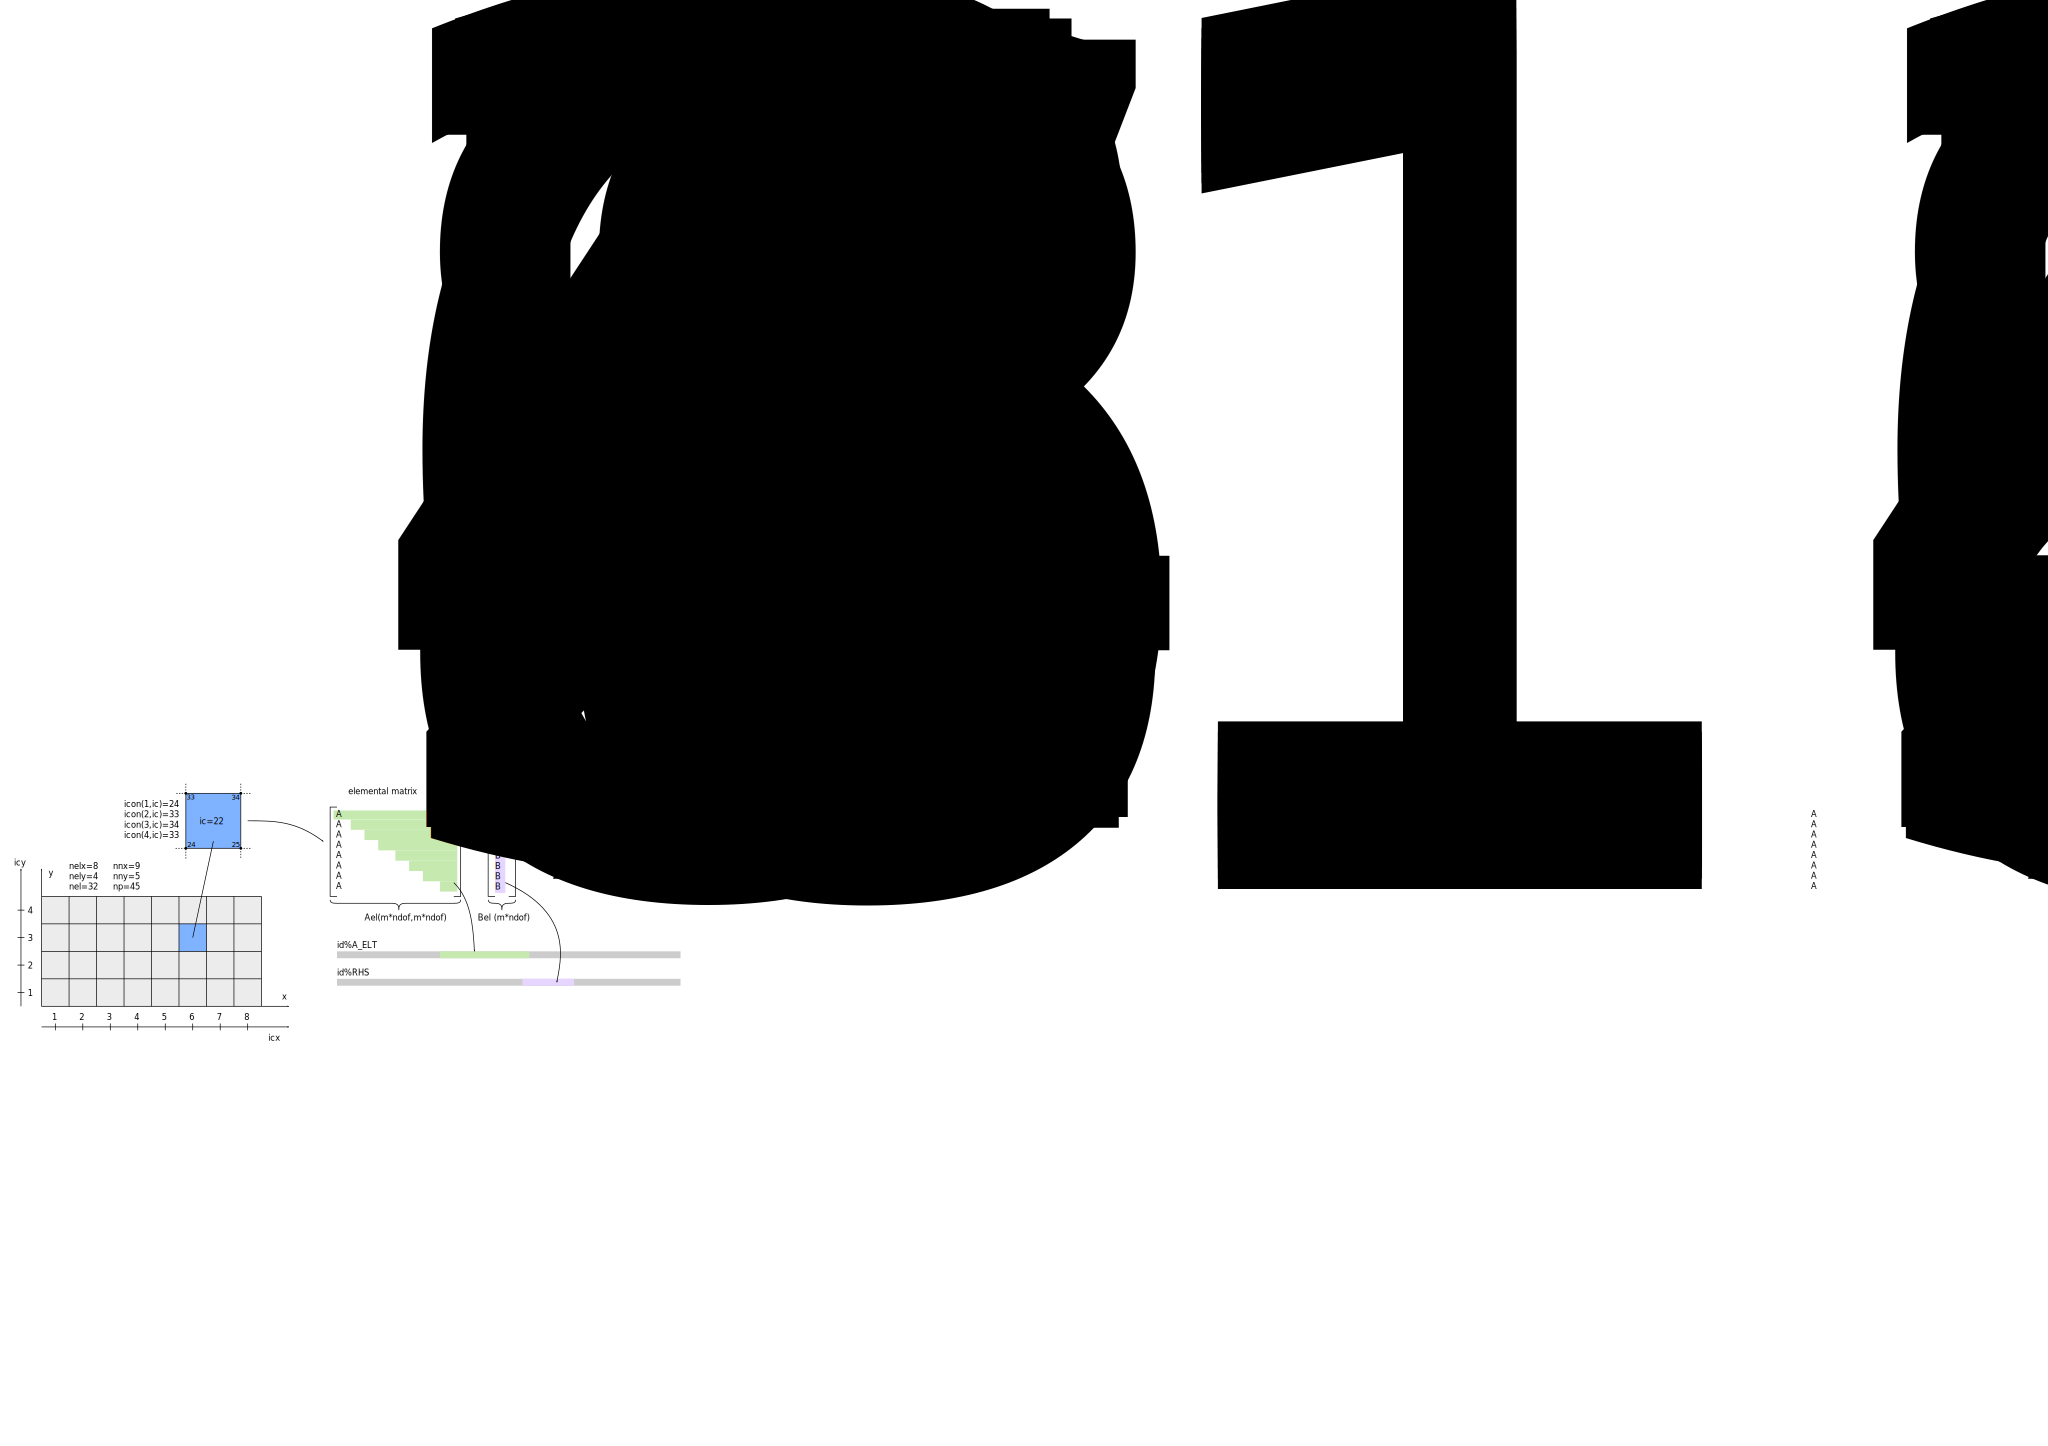
\includegraphics[width=7cm]{python_codes/fieldstone_12/results/rand/grid}
\end{center}

We repeat the same exercise as before on such a mesh and look at the errors

\begin{center}
\includegraphics[width=10cm]{python_codes/fieldstone_12/results/rand/errors}
\end{center}

Rather surprisingly we find that $q_1$ proves to be the most accurate of all pressures and it converges
with $h^{1.5}$ as before. Because checkerboard modes are triggered the convergence of the elemental 
pressure is more chaotic but on average linear. 
The $q_2$ and $q_3$ fields seem to unexpectedly stop converging above a given resolution. 

\begin{center}
\includegraphics[width=7cm]{python_codes/fieldstone_12/results/rand/pressure}
\includegraphics[width=7cm]{python_codes/fieldstone_12/results/rand/pressure_error}\\
\includegraphics[width=7cm]{python_codes/fieldstone_12/results/rand/p_error}
\includegraphics[width=7cm]{python_codes/fieldstone_12/results/rand/q1_error}\\
\includegraphics[width=7cm]{python_codes/fieldstone_12/results/rand/q2_error}
\includegraphics[width=7cm]{python_codes/fieldstone_12/results/rand/q3_error}\\
\includegraphics[width=7cm]{python_codes/fieldstone_12/results/rand/q4_error}
\includegraphics[width=7cm]{python_codes/fieldstone_12/results/rand/q5_error}\\
{\captionfont Left: pressure fields as a function of the $x$-coordinate.} 
\end{center}

\begin{center}
\includegraphics[width=7cm]{python_codes/fieldstone_12/results/rand/erq1}
\includegraphics[width=7cm]{python_codes/fieldstone_12/results/rand/erq2}\\
\includegraphics[width=7cm]{python_codes/fieldstone_12/results/rand/erq3}
\includegraphics[width=7cm]{python_codes/fieldstone_12/results/rand/erq4}\\
\includegraphics[width=7cm]{python_codes/fieldstone_12/results/rand/erq5}
\includegraphics[width=7cm]{python_codes/fieldstone_12/results/rand/erq6}
\end{center}



